\chapter[Complete results]{Complete results}\label{ch:app_results}
%************************************************

%\renewcommand{\thefigure}{A.2.1.\arabic{figure}}
%\setcounter{figure}{0}

%\renewcommand{\thetable}{A.2.1.\arabic{table}}
%\setcounter{table}{0}
\hrulefill

\section*{Experiment 1: Performance against baselines} \label{app:ex1_cont}

\subsection*{Best performance for each metric across scenarios (continued)}
\begin{landscape}
\begin{table}[]
\centering
\caption[Performance of models and baselines during training (continued).]{Performance of models and baselines during training (continued). Bold values correspond to the best performance for each metric. \textit{C}, \textit{B} and \textit{P} designate car, bicycle and pedestrian-specific results, respectively. $\Sigma$ represents combined results.}
\label{tab:perf_part2}
\begin{tabular}{lccccccc}
\toprule
\multicolumn{1}{c}{\multirow{2}{*}{\textbf{\begin{tabular}[c]{@{}c@{}}Single\\ intersection\end{tabular}}}} & \multicolumn{4}{c}{\begin{tabular}[c]{@{}c@{}}Throughput [ents./h]\end{tabular}} & \multicolumn{3}{c}{\begin{tabular}[c]{@{}c@{}}Never arrived [ents.]\end{tabular}} \\
\cmidrule(r){2-5} \cmidrule(l){6-8}
\multicolumn{1}{c}{} & C & B & P & $\Sigma$ & C & B & \textbf{P} \\
\midrule
Stochastic & 2888.6 & \textbf{867} & \textbf{742} & 4497.6 & 69.6 & \textbf{0} & \textbf{0} \\
Max Pressure & 3306.2 & 844.6 & \textbf{742} & 4884.4 & 82.8 & 0.4 & \textbf{0} \\
Max Wave & 3115.4 & 835 & \textbf{742} & 4692.4 & 85 & 26.8 & \textbf{0} \\
Fixed time 20 & 3607 & \textbf{867} & \textbf{742} & 5216 & 33.4 & \textbf{0} & \textbf{0} \\
Fixed time 40 & 3602.8 & \textbf{867} & \textbf{742} & 5211.8 & \textbf{32} & \textbf{0} & \textbf{0} \\
IDQN & 3829.4 & \textbf{867} & \textbf{742} & 5438.2 & 41 & \textbf{0} & \textbf{0} \\
IDQN MM & 3504.6 & \textbf{867} & \textbf{742} & 5113.6 & 42.4 & \textbf{0} & \textbf{0} \\
MPLight & 3436.6 & \textbf{867} & \textbf{742} & 5045.6 & 41.6 & \textbf{0} & \textbf{0} \\
MPLight MM & 3758.8 & \textbf{867} & \textbf{742} & 5367.8 & 33 & \textbf{0} & \textbf{0} \\
IPPO & 3619 & \textbf{867} & \textbf{742} & 5228 & 33 & \textbf{0} & \textbf{0} \\
FMA2C & \textbf{4772} & \textbf{867} & \textbf{742} & \textbf{6381} & \textbf{32} & \textbf{0} & \textbf{0} \\
\midrule
\textbf{Corridor} &  &  &  &  &  &  &  \\ \midrule
Max Pressure & 2111 & 10176 & 3616 & 15885 & 34 & 449 & 26 \\
Max Wave & 2040 & 10077 & 3630 & 15721 & 35 & 466 & 12 \\
Fixed time 20 & 3202 & 12506 & \textbf{3642} & 19346 & 18 & 305 & \textbf{0} \\
Fixed time 40 & 3204 & 12477 & \textbf{3642} & 19305 & 19 & 357 & \textbf{0} \\
IDQN & 3193 & 11962 & \textbf{3642} & 18639 & \textbf{1} & 193 & \textbf{0} \\
IDQN MM & 3198 & 12703 & \textbf{3642} & 19538 & 16 & 136 & \textbf{0} \\
MPLight & 3195 & 12391 & \textbf{3642} & 19170 & 11 & 171 & \textbf{0} \\
IPPO & 3146 & 12157 & \textbf{3642} & 18954 & 9 & 277 & \textbf{0} \\
FMA2C & \textbf{3213} & \textbf{12974} & \textbf{3642} & \textbf{19848} & 18 & \textbf{57} & \textbf{0} \\ \bottomrule
\end{tabular}
\end{table}
\end{landscape}

\subsection*{Additional plots}
\subsubsection{Single intersection scenario}

\begin{figure}
  \centering
  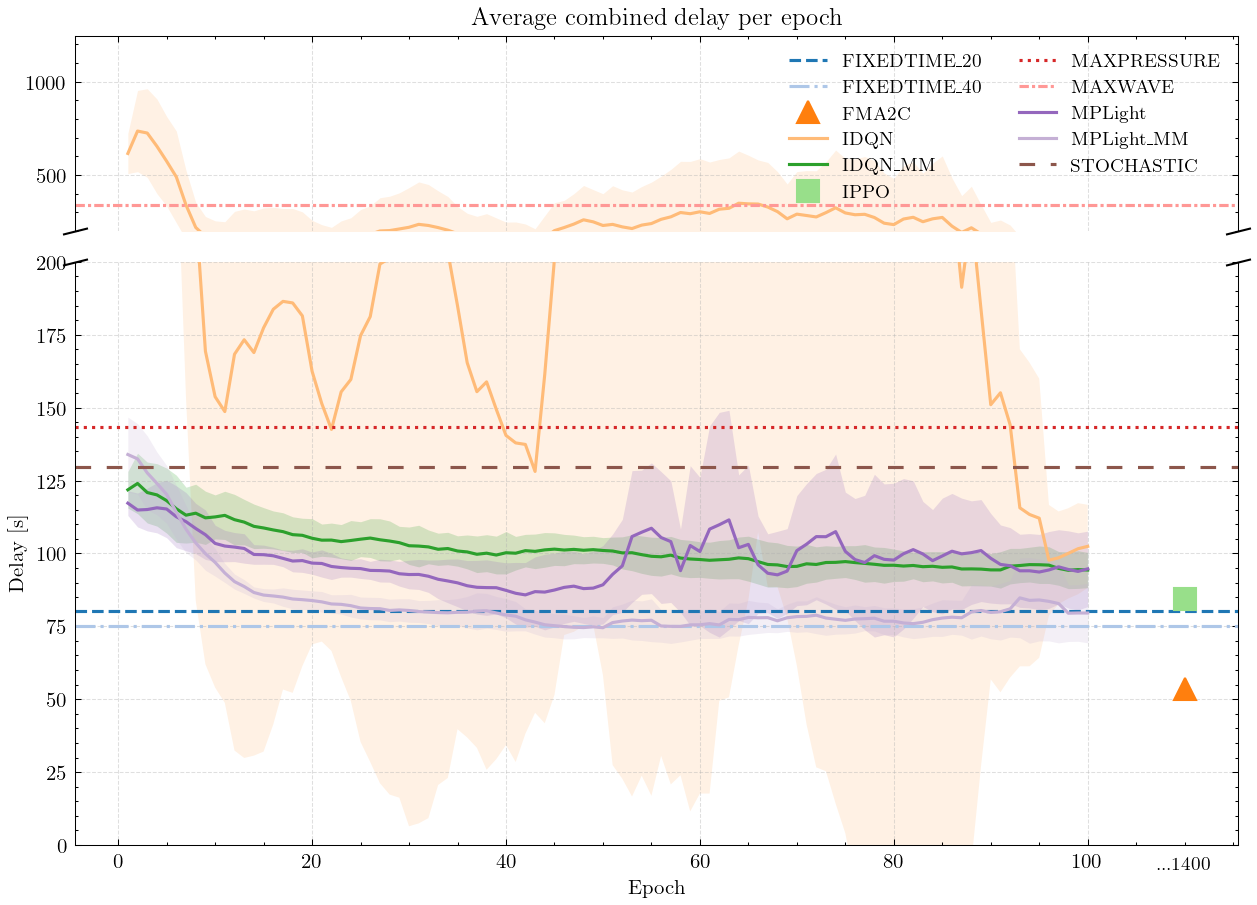
\includegraphics[width=\linewidth]{Figures/chapter04/plotsj1/timeLoss.png}
  \captionof{figure}{Average combined time loss per epoch.} \label{fig:timeLoss_j1}
\end{figure}%
\begin{figure}
  \centering
  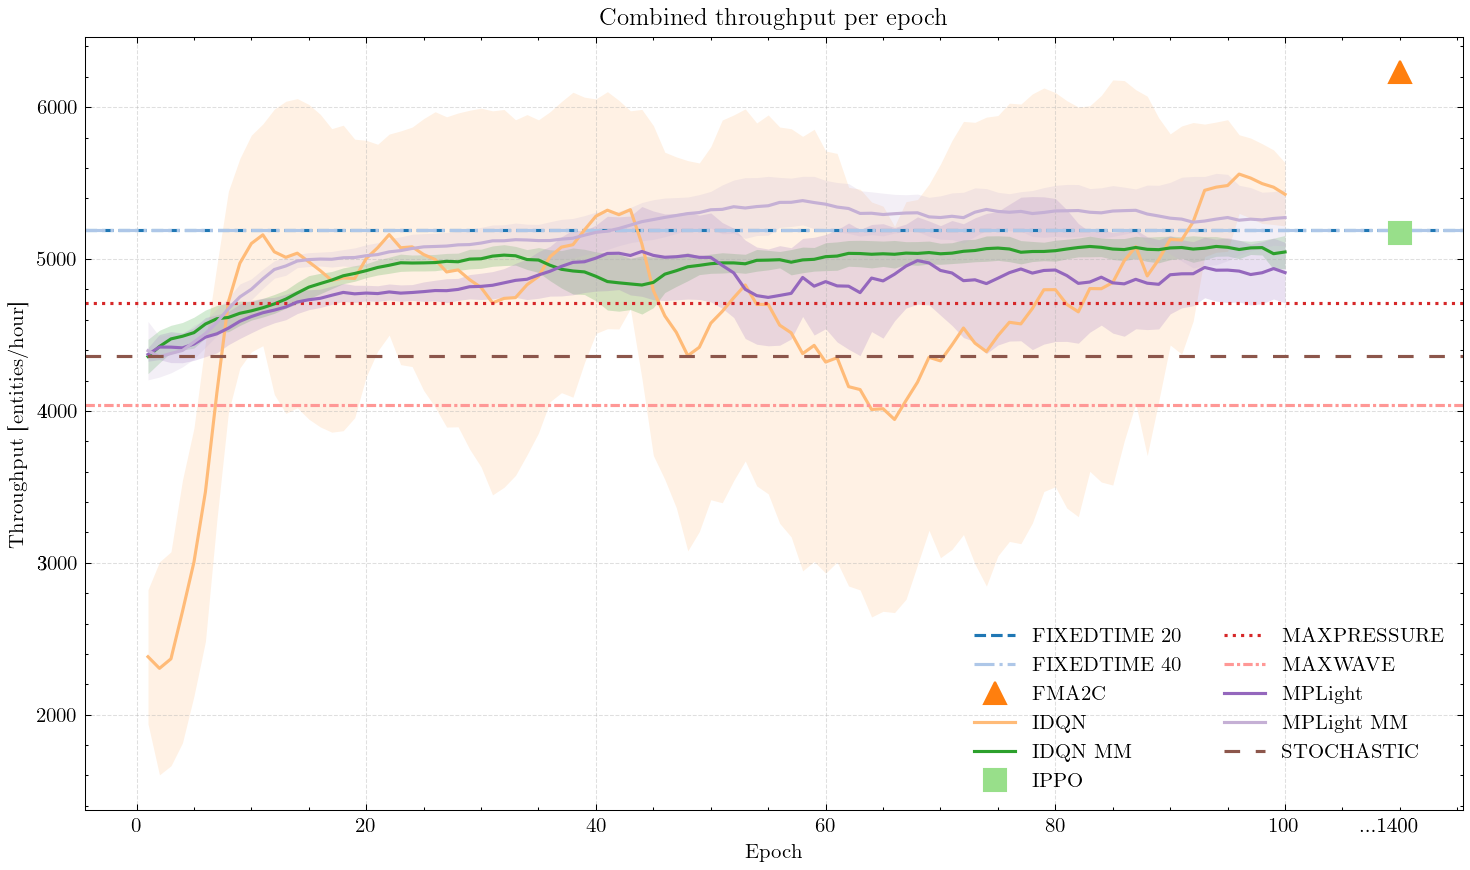
\includegraphics[width=\linewidth]{Figures/chapter04/plotsj1/throughput_combined.png}
  \caption{Single intersection: average combined throughput per epoch.} \label{fig:throughput_j1}
\end{figure}

\begin{figure}
  \centering
  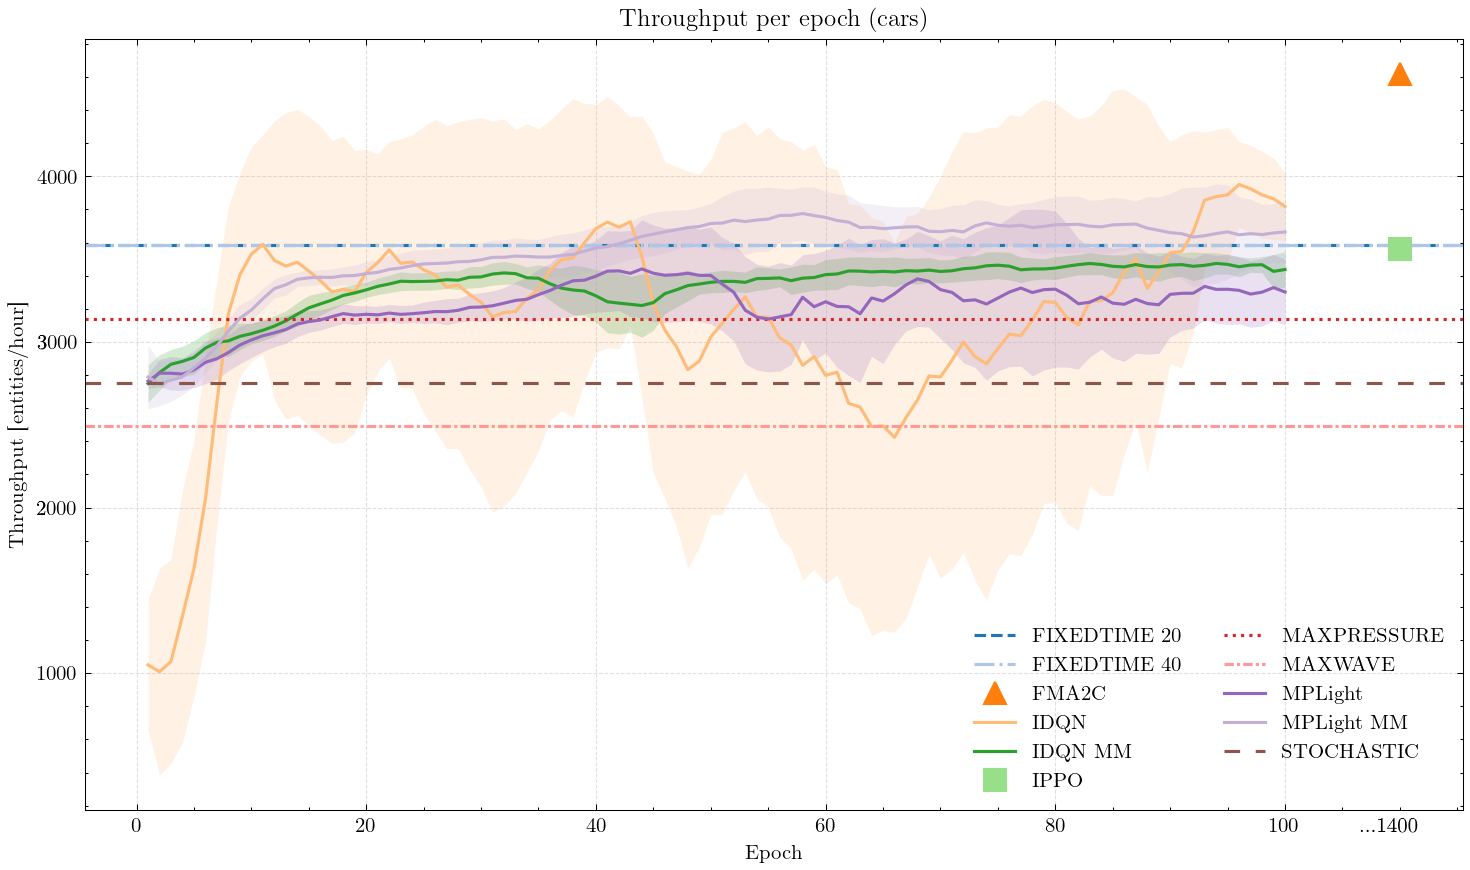
\includegraphics[width=\linewidth]{Figures/chapter04/plotsj1/throughput_car.png}
  \caption{Single intersection: average car throughput per epoch.} \label{fig:throughput_cars_j1}
\end{figure}%
\begin{figure}
  \centering
  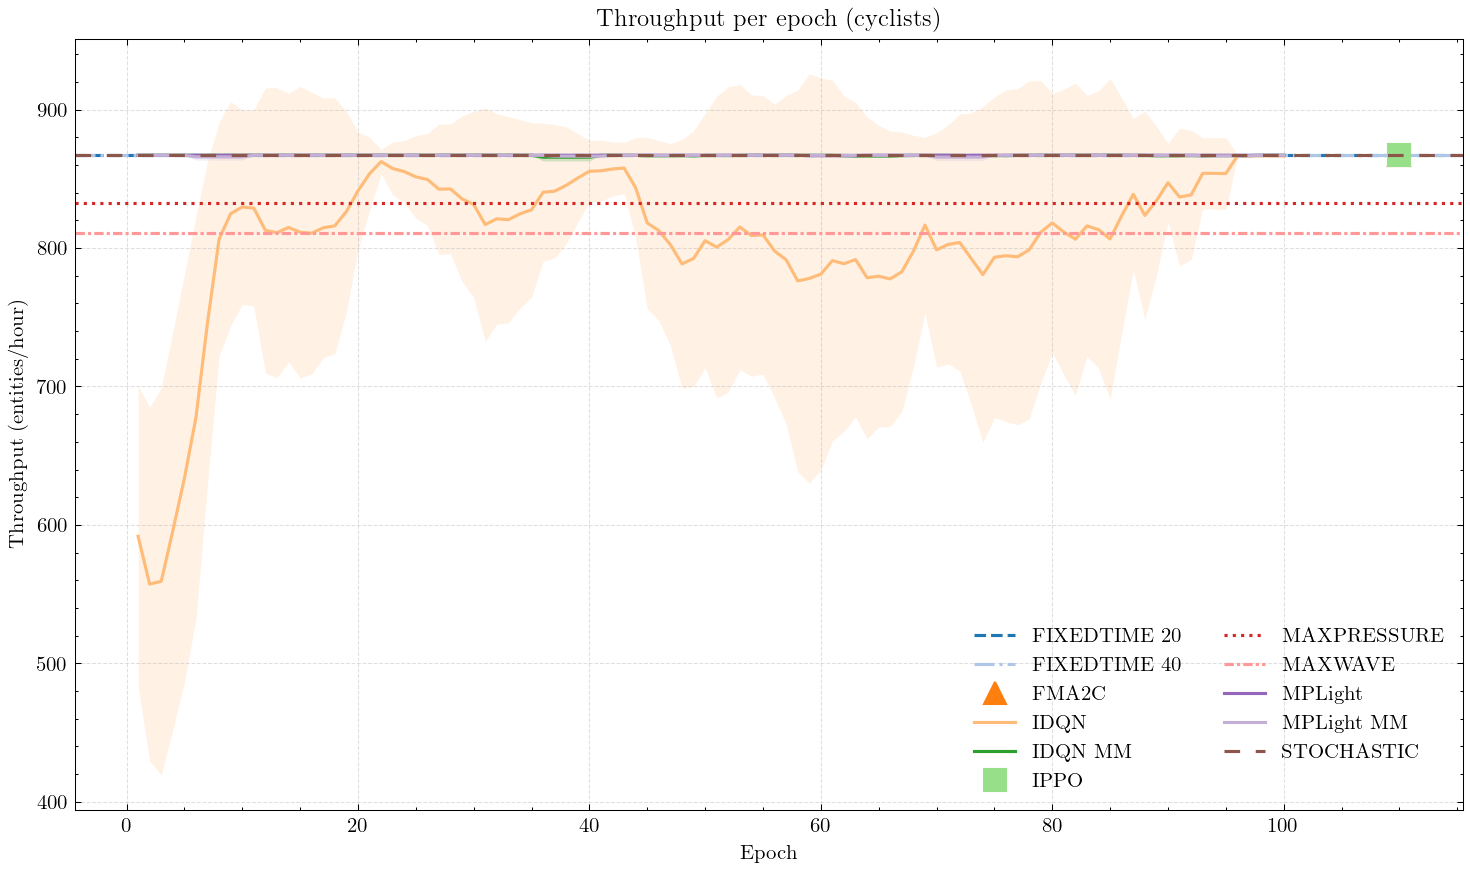
\includegraphics[width=\linewidth]{Figures/chapter04/plotsj1/throughput_bike.png}
  \caption{Single intersection: average bicycle throughput per epoch.} \label{fig:throughput_bikes_j1}
\end{figure}

\begin{figure}
  \centering
  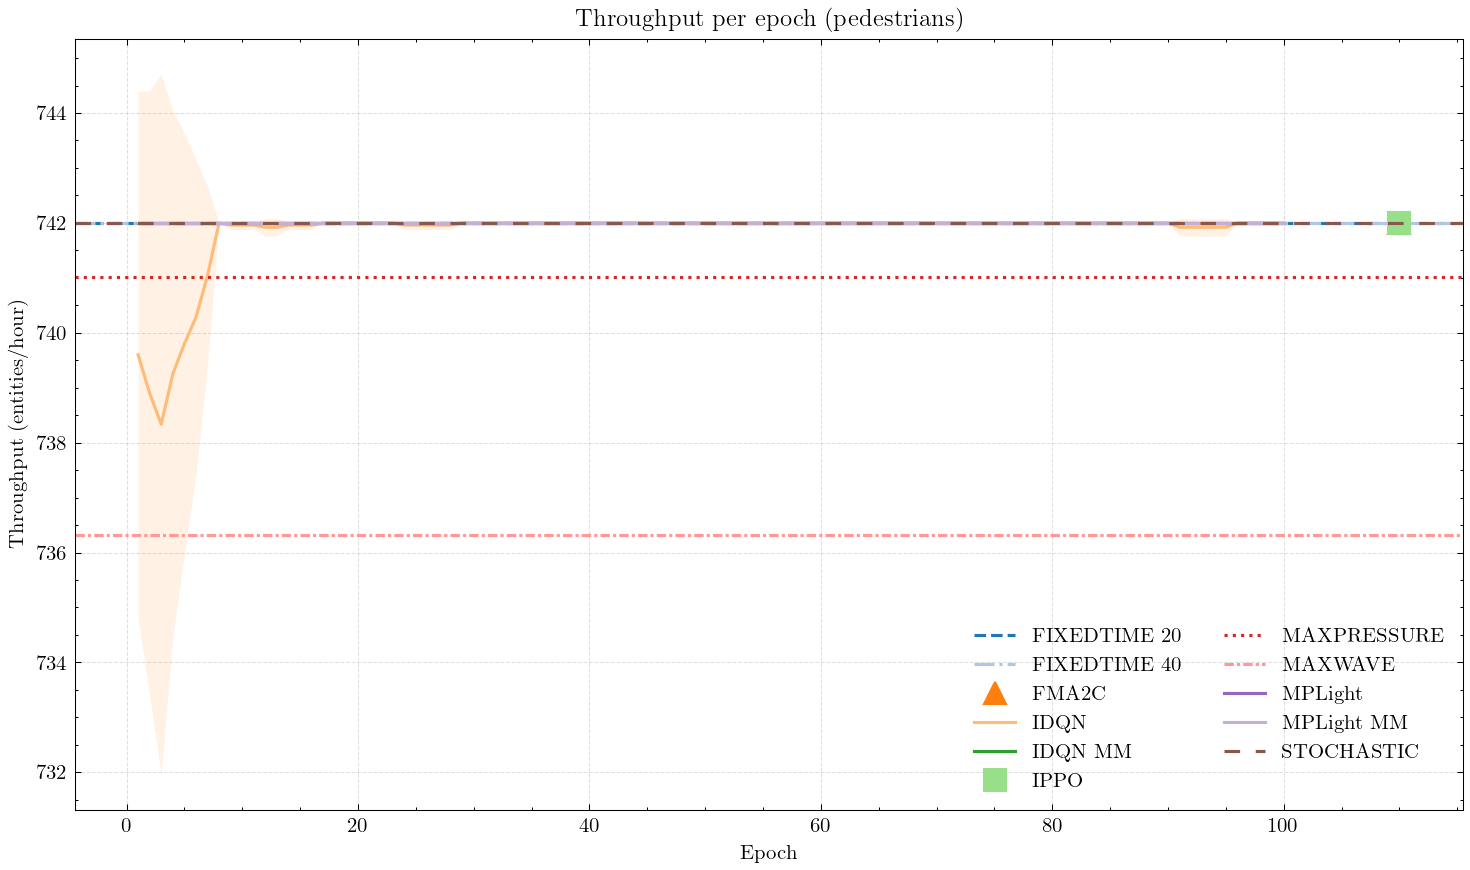
\includegraphics[width=\linewidth]{Figures/chapter04/plotsj1/throughput_pedestrian.png}
  \caption{Single intersection: average pedestrian throughput per epoch.} \label{fig:throughput_pedestrians_j1}
\end{figure}%
\begin{figure}
  \centering
  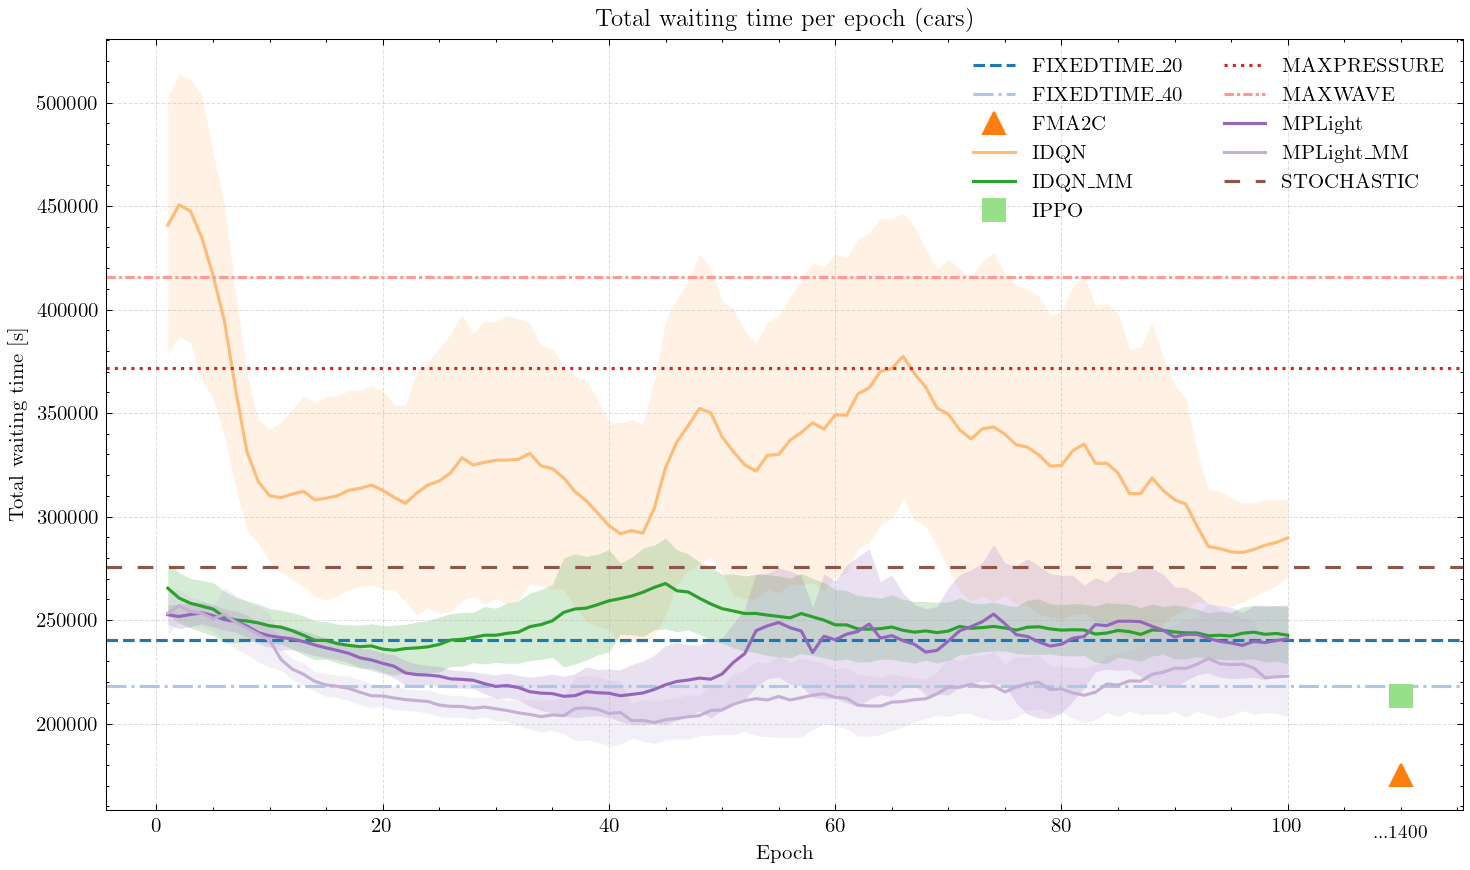
\includegraphics[width=\linewidth]{Figures/chapter04/plotsj1/wait_total_smoothed_car.png}
  \caption{Single intersection: accumulated waiting time, for cars, per epoch.} \label{fig:total_wait_cars_j1}
\end{figure}

\begin{figure}
  \centering
  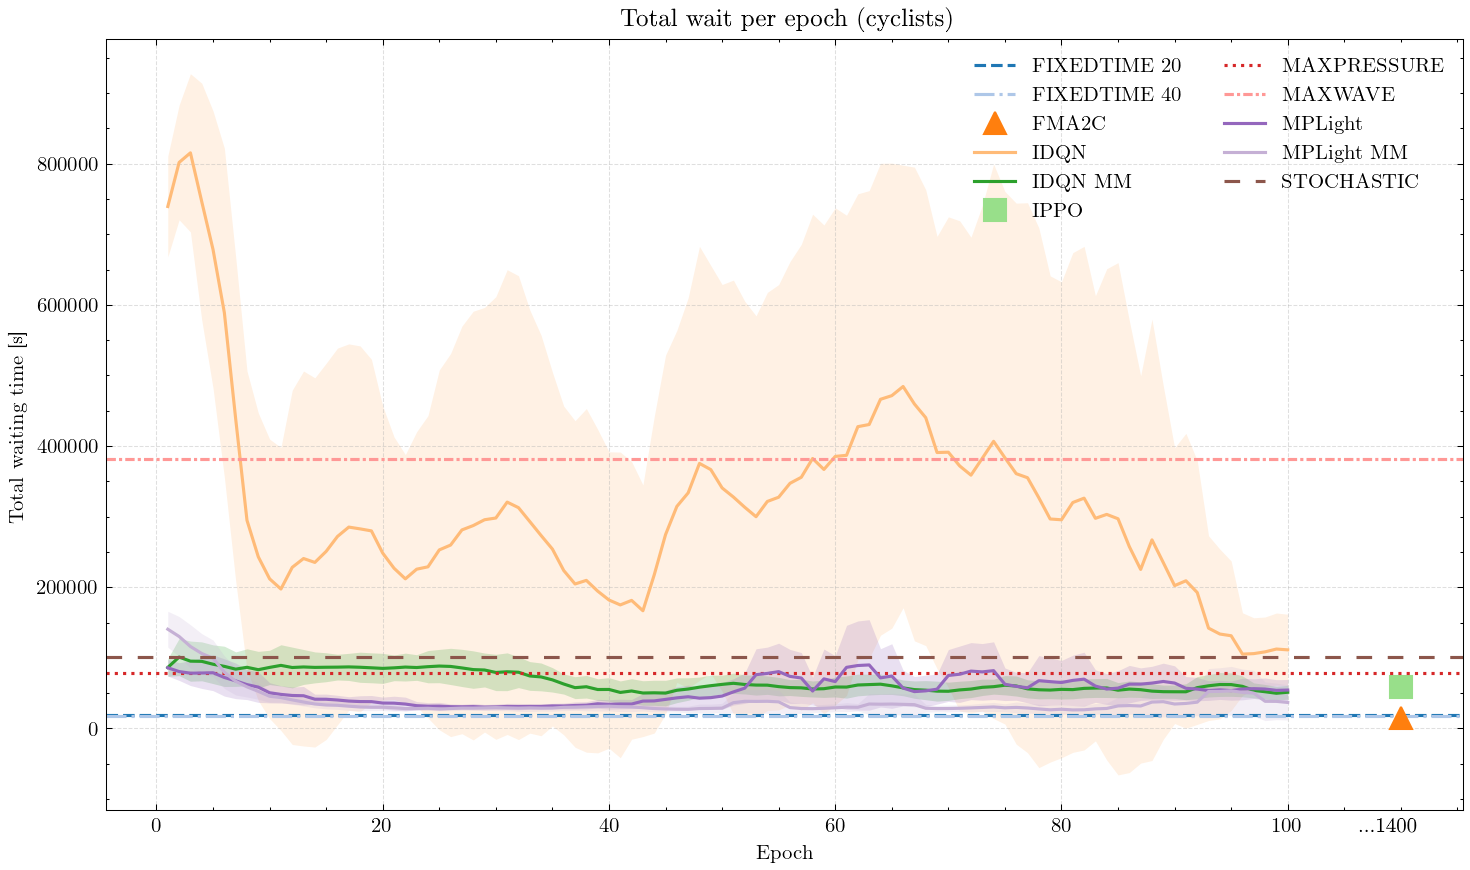
\includegraphics[width=\linewidth]{Figures/chapter04/plotsj1/wait_total_smoothed_bike.png}
  \caption{Single intersection: accumulated waiting time, for bicycles, per epoch.} \label{fig:total_wait_bikes_j1}
\end{figure}%
\begin{figure}
  \centering
  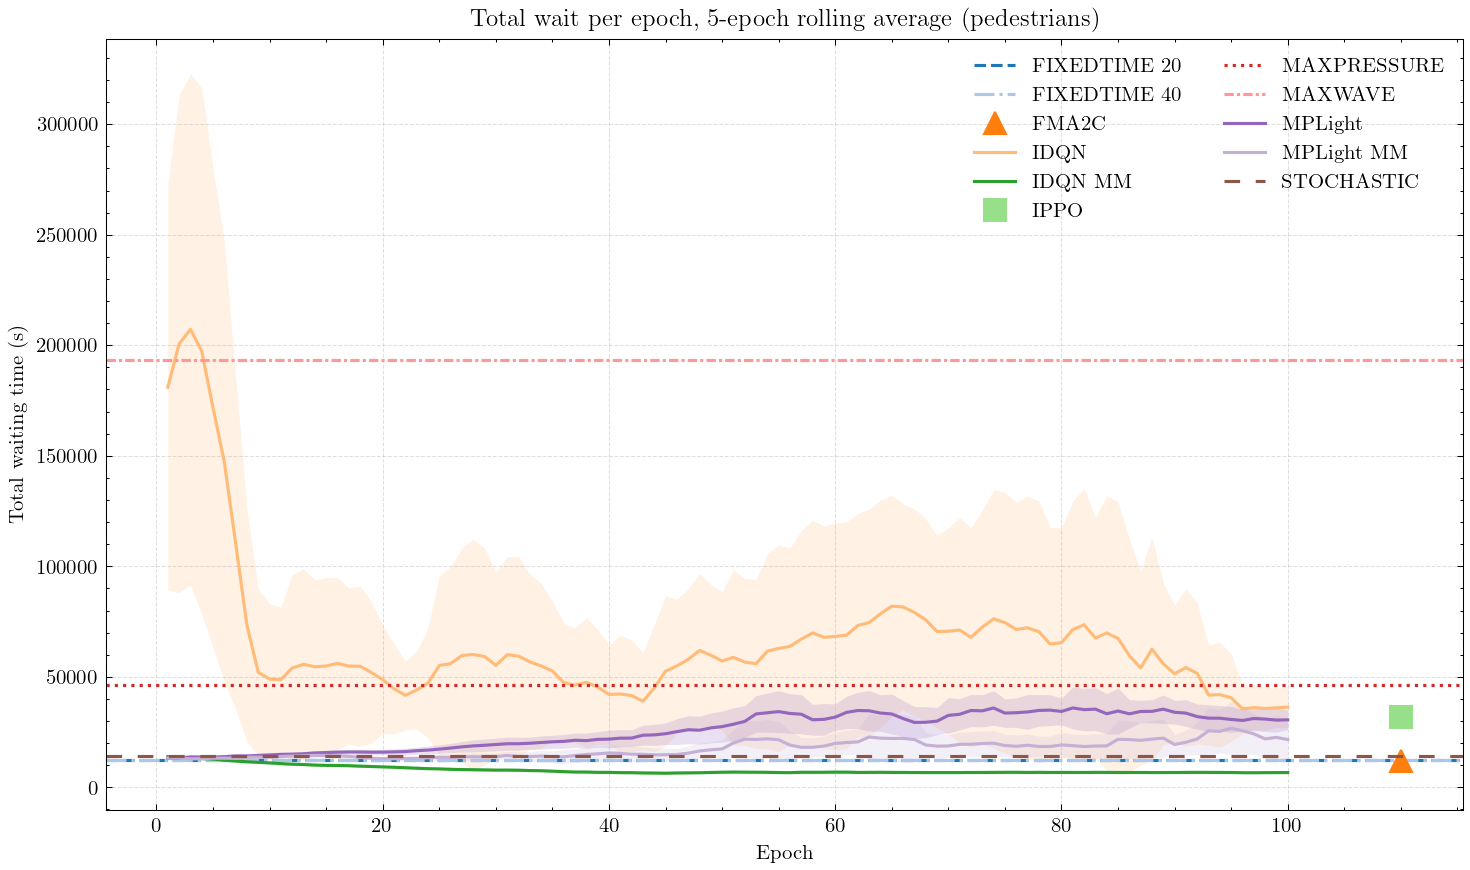
\includegraphics[width=\linewidth]{Figures/chapter04/plotsj1/wait_total_smoothed_pedestrian.png}
  \caption{Single intersection: accumulated waiting time, for pedestrians, per epoch.} \label{fig:total_wait_pedestrians_j1}
\end{figure}

\begin{figure}
  \centering
  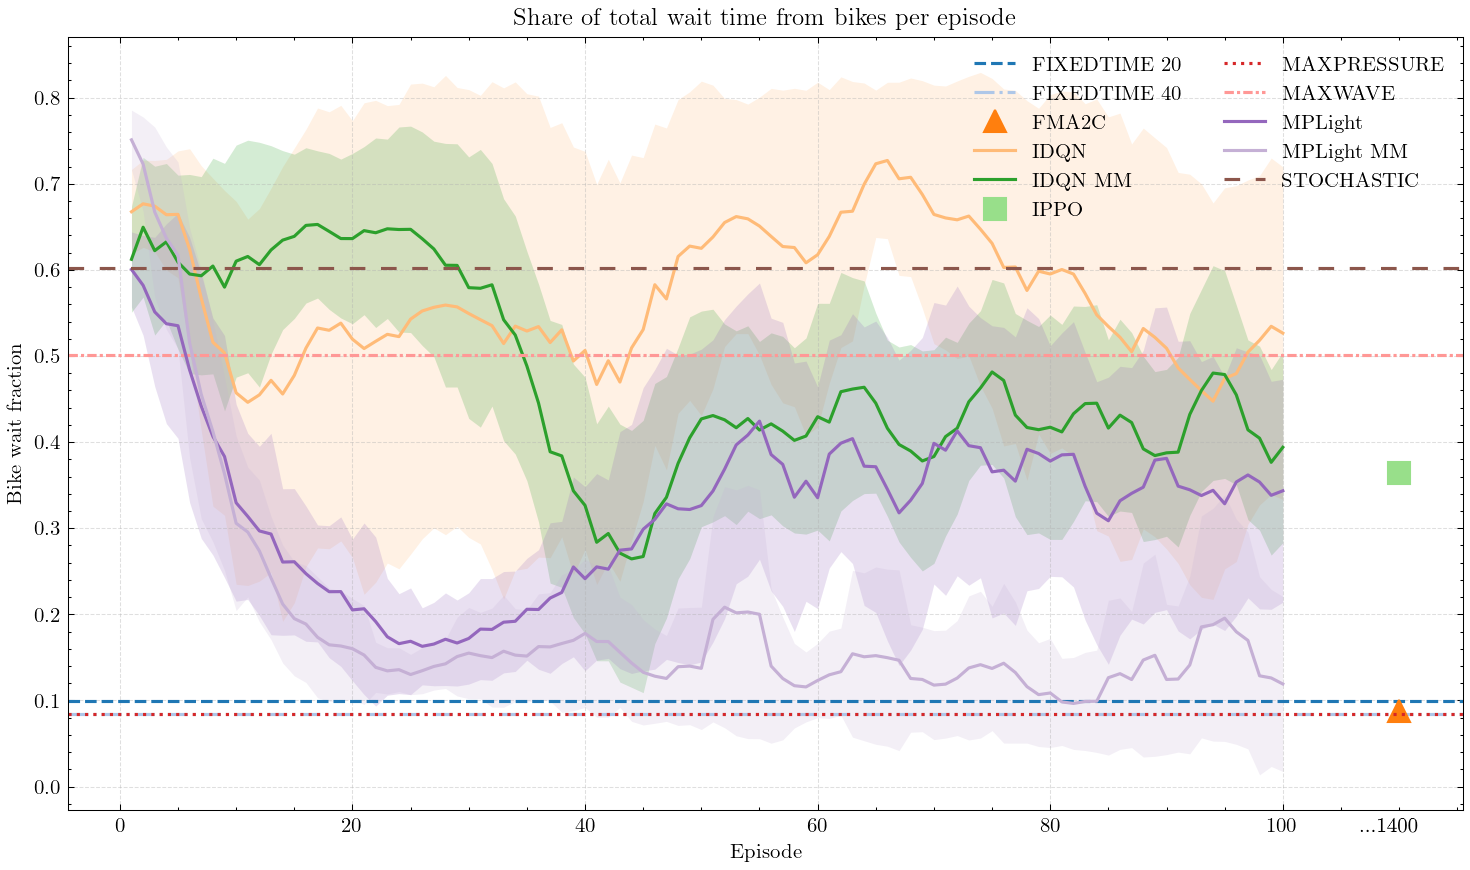
\includegraphics[width=\linewidth]{Figures/chapter04/plotsj1/episode_wait_frac_bike.png}
  \caption{Single intersection: fraction of waiting time due to bicycles, per epoch.} \label{fig:frac_wait_bikes_j1}
\end{figure}%
\begin{figure}
  \centering
  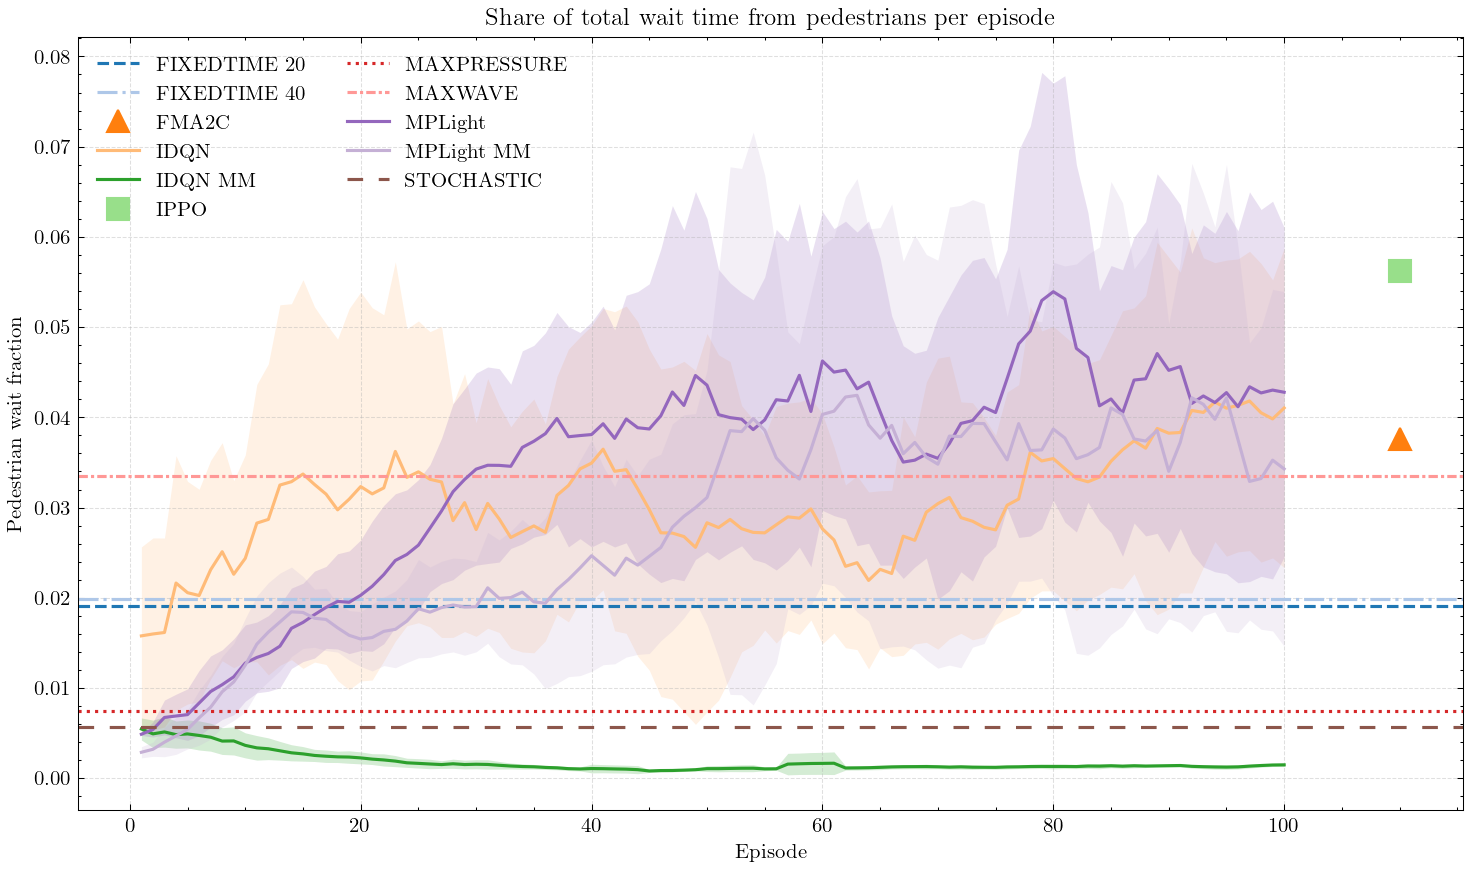
\includegraphics[width=\linewidth]{Figures/chapter04/plotsj1/episode_wait_frac_ped.png}
  \caption{Single intersection: fraction of waiting time due to pedestrians, per epoch.} \label{fig:frac_wait_pedestrians_j1}
\end{figure}

\subsubsection{Corridor scenario}

\begin{figure}
  \centering
  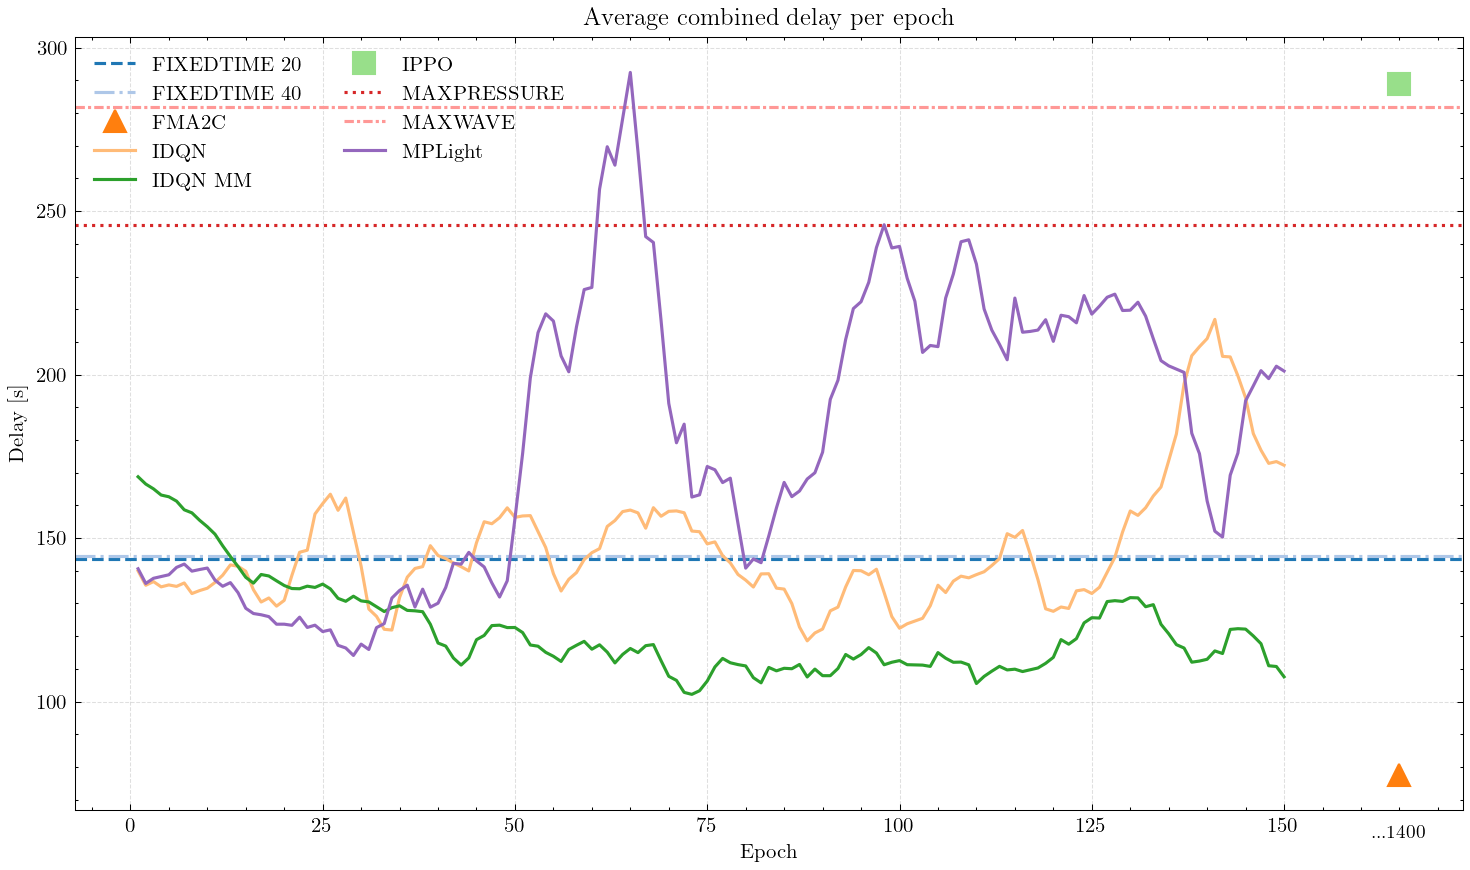
\includegraphics[width=\linewidth]{Figures/chapter04/plotsc2/timeLoss.png}
  \captionof{figure}{Corridor: average combined time loss per epoch.} \label{fig:timeLoss_c2}
\end{figure}%
\begin{figure}
  \centering
  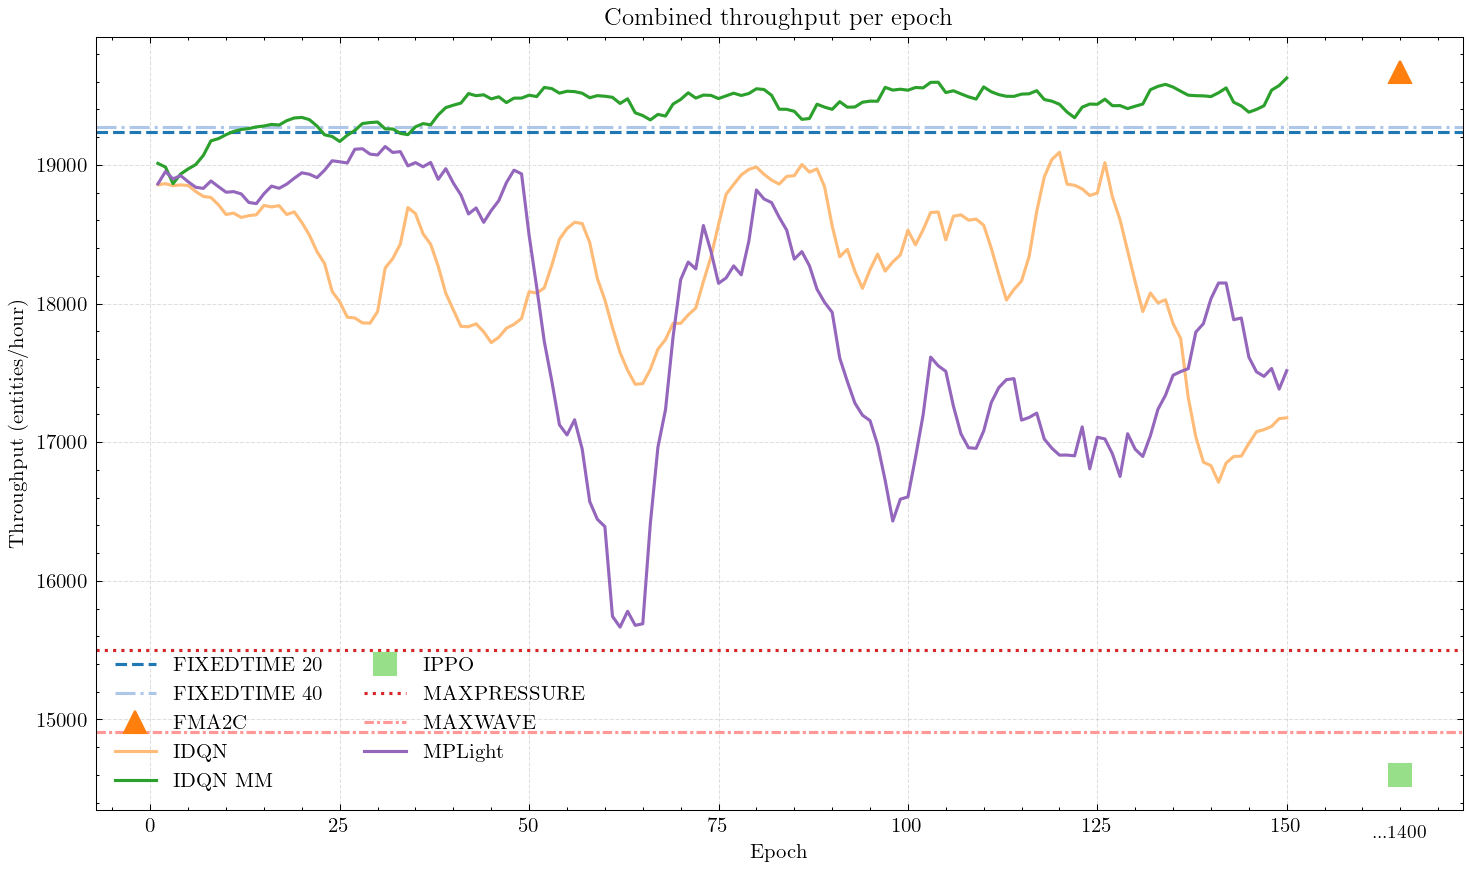
\includegraphics[width=\linewidth]{Figures/chapter04/plotsc2/throughput_combined.png}
  \caption{Corridor: average combined throughput per epoch.} \label{fig:throughput_c2}
\end{figure}

\begin{figure}
  \centering
  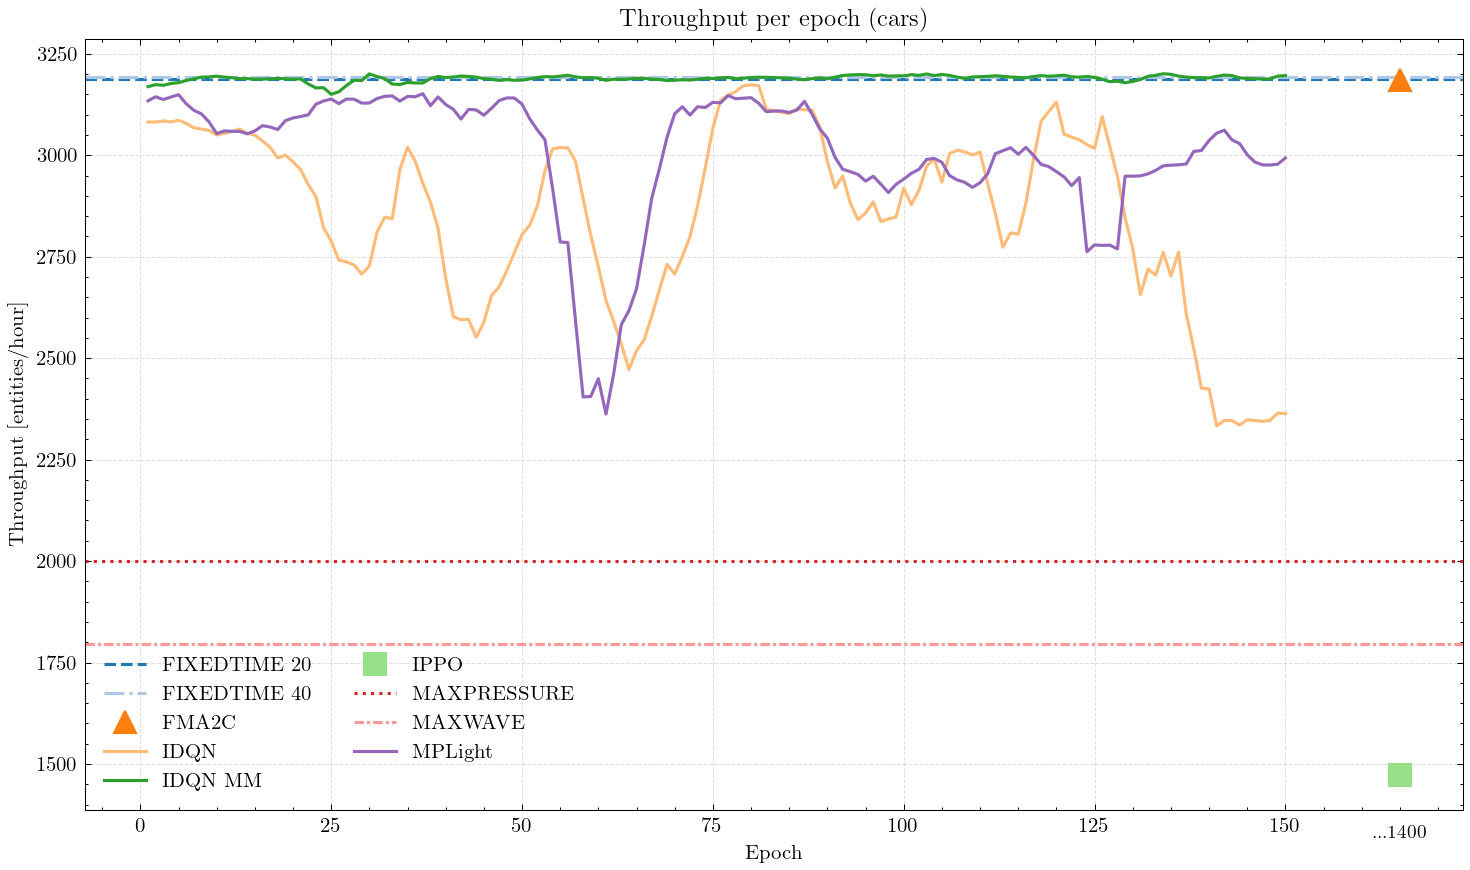
\includegraphics[width=\linewidth]{Figures/chapter04/plotsc2/throughput_car.png}
  \caption{Corridor: average car throughput per epoch.} \label{fig:throughput_cars_c2}
\end{figure}%
\begin{figure}
  \centering
  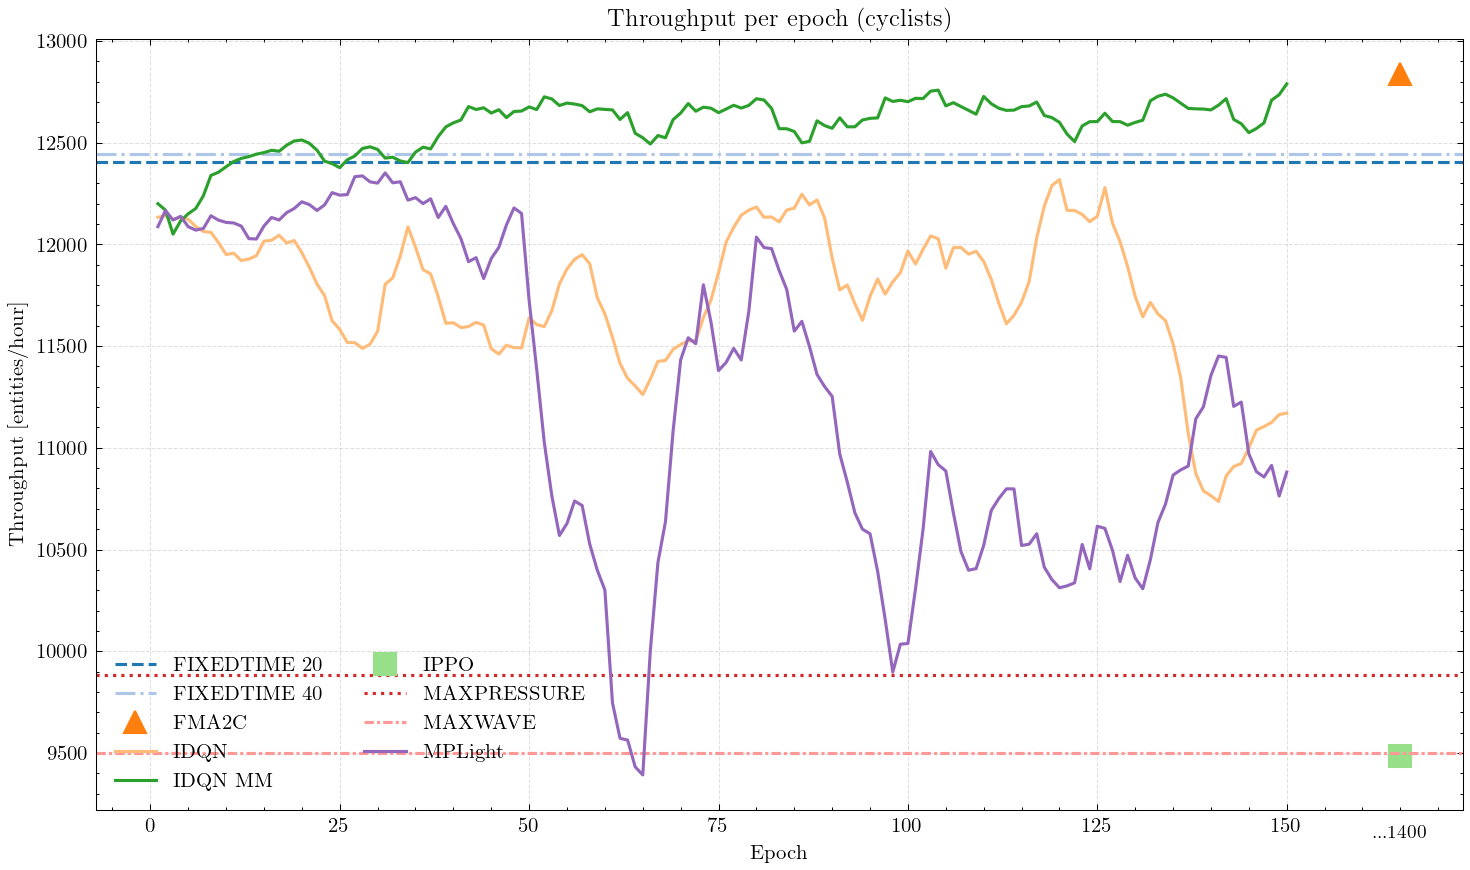
\includegraphics[width=\linewidth]{Figures/chapter04/plotsc2/throughput_bike.png}
  \caption{Corridor: average bicycle throughput per epoch.} \label{fig:throughput_bikes_c2}
\end{figure}

\begin{figure}
  \centering
  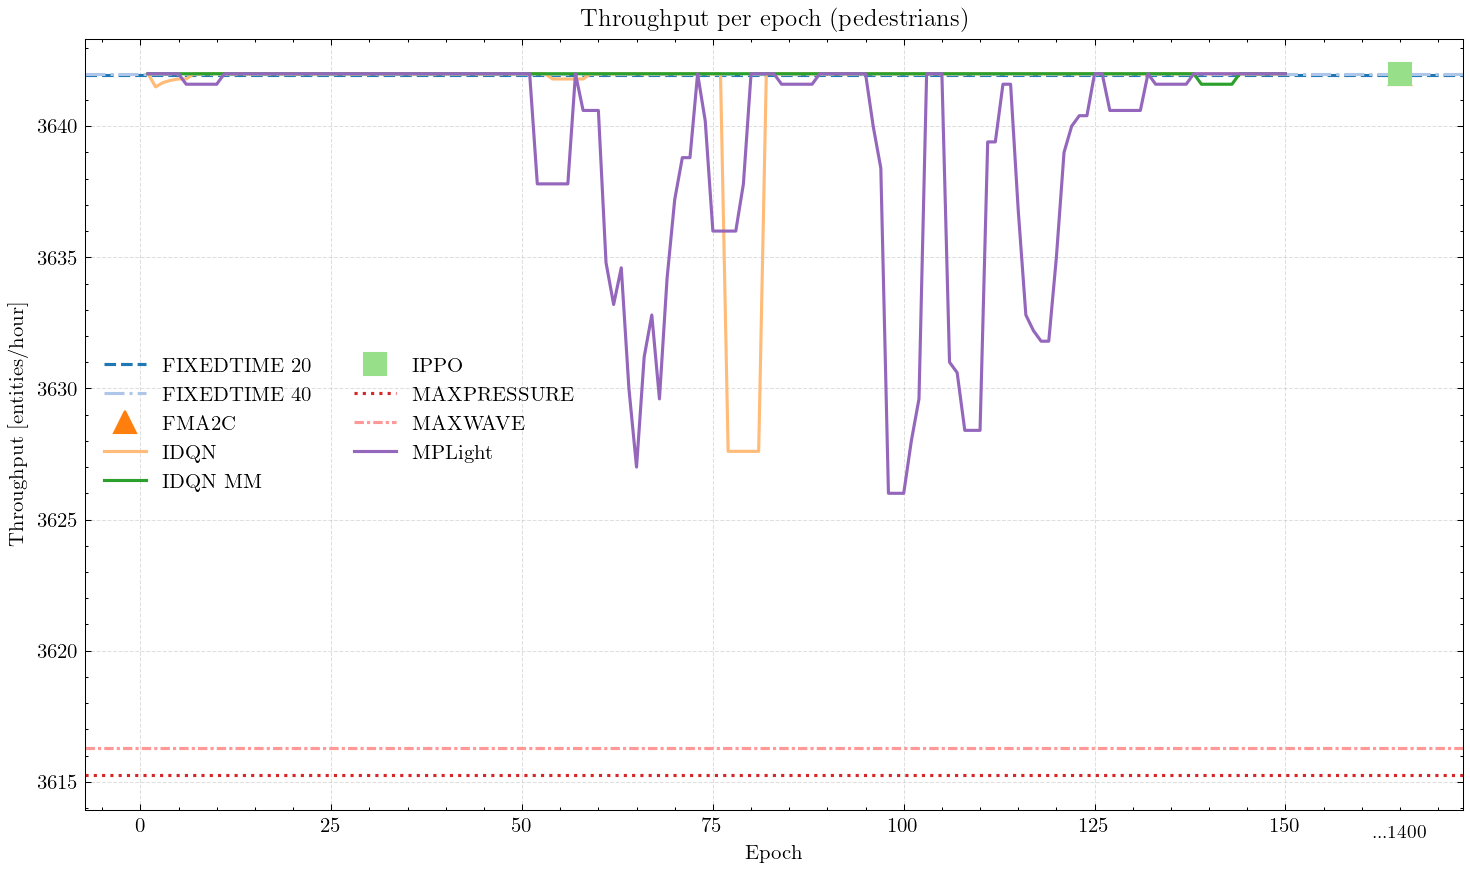
\includegraphics[width=\linewidth]{Figures/chapter04/plotsc2/throughput_pedestrian.png}
  \caption{Corridor: average pedestrian throughput per epoch.} \label{fig:throughput_pedestrians_c2}
\end{figure}%
\begin{figure}
  \centering
  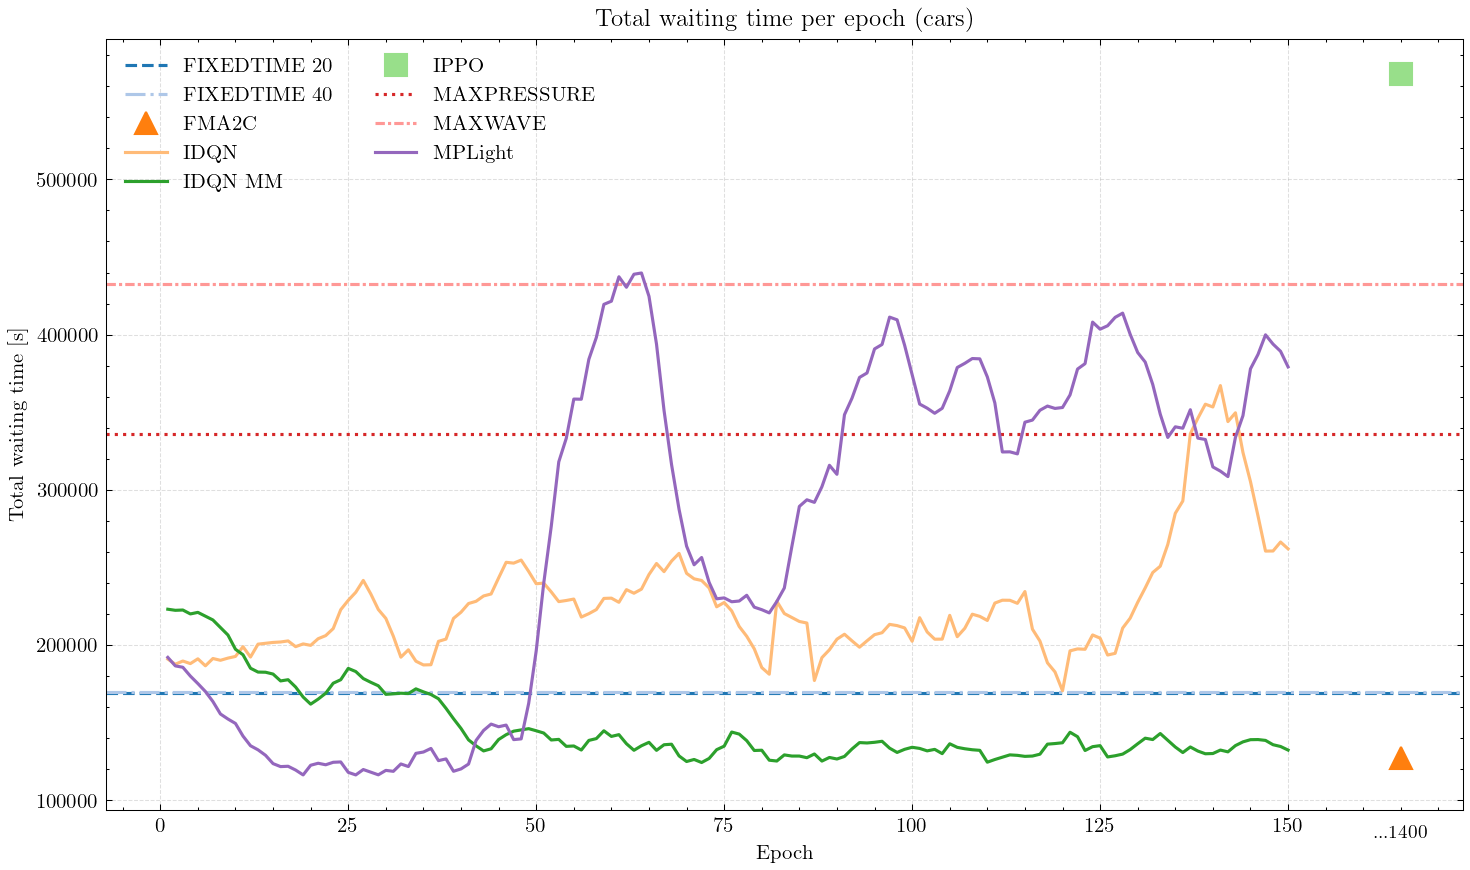
\includegraphics[width=\linewidth]{Figures/chapter04/plotsc2/wait_total_smoothed_car.png}
  \caption{Corridor: accumulated waiting time, for cars, per epoch.} \label{fig:total_wait_cars_c2}
\end{figure}

\begin{figure}
  \centering
  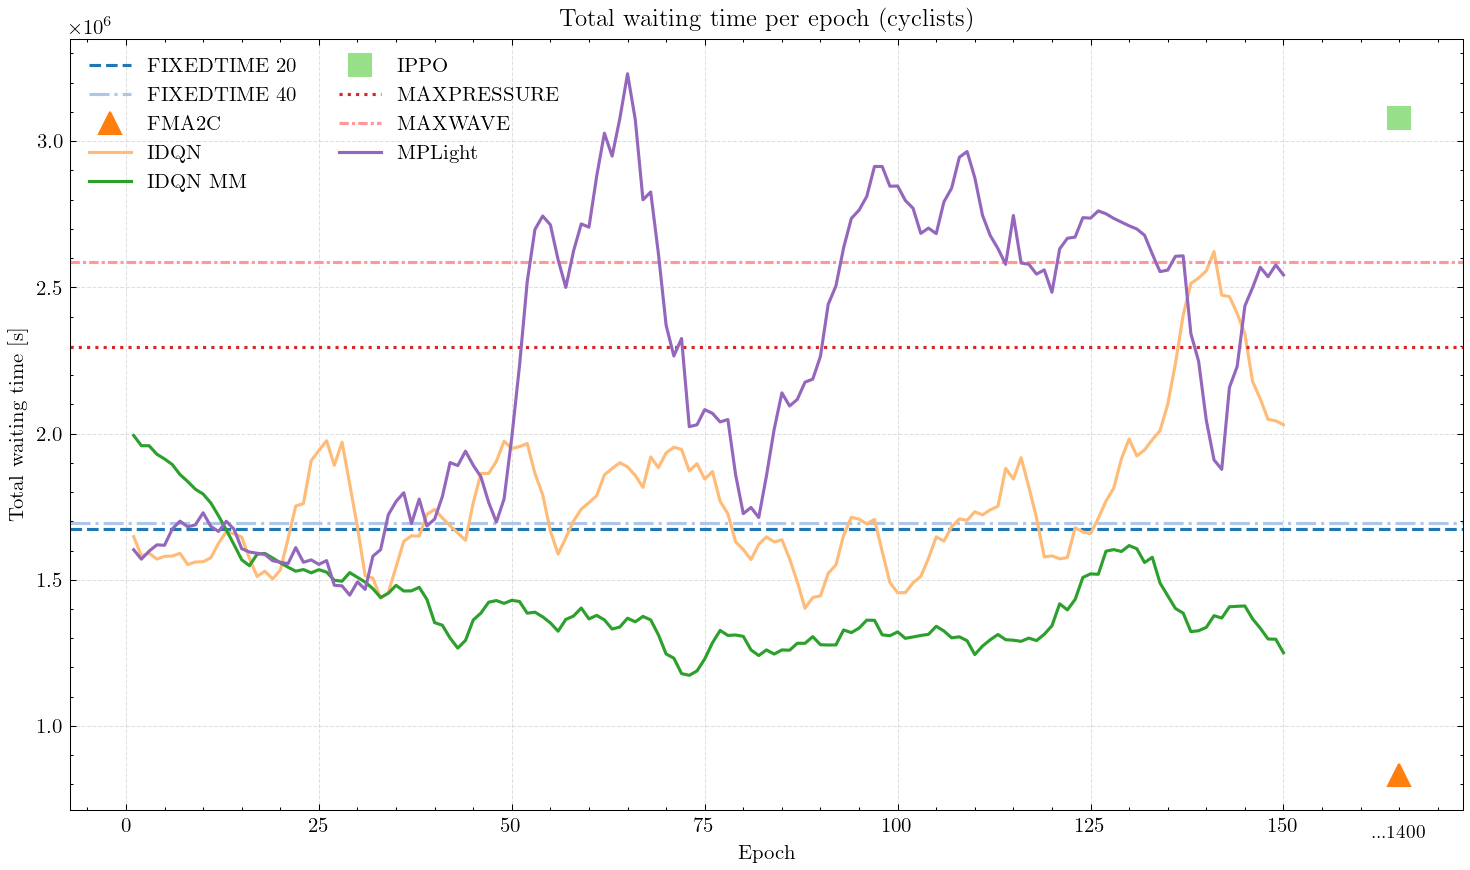
\includegraphics[width=\linewidth]{Figures/chapter04/plotsc2/wait_total_smoothed_bike.png}
  \caption{Corridor: accumulated waiting time, for bicycles, per epoch.} \label{fig:total_wait_bikes_c2}
\end{figure}%
\begin{figure}
  \centering
  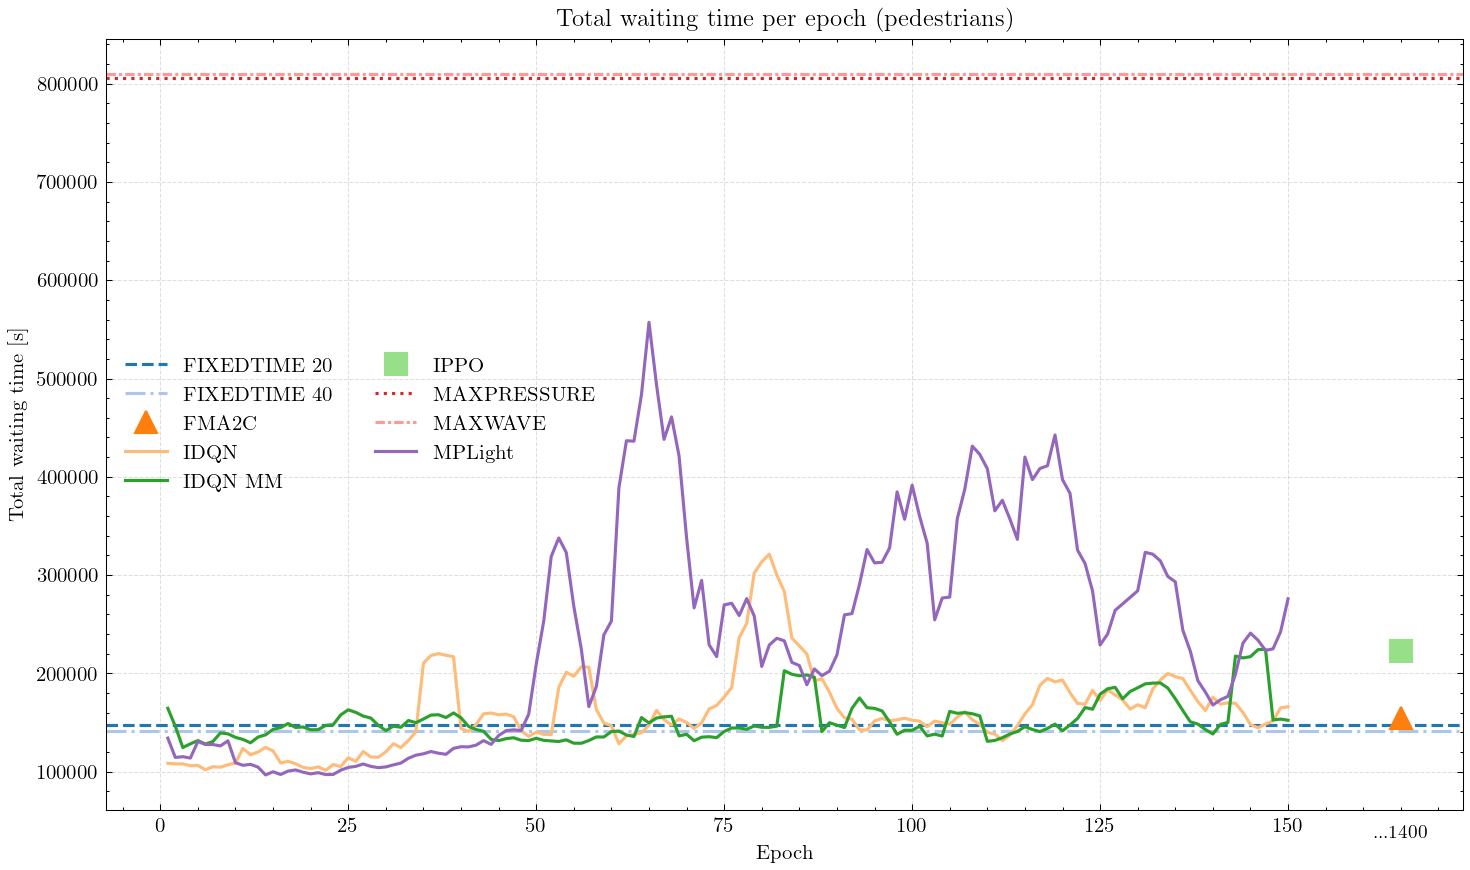
\includegraphics[width=\linewidth]{Figures/chapter04/plotsc2/wait_total_smoothed_pedestrian.png}
  \caption{Corridor: accumulated waiting time, for pedestrians, per epoch.} \label{fig:total_wait_pedestrians_c2}
\end{figure}

\begin{figure}
  \centering
  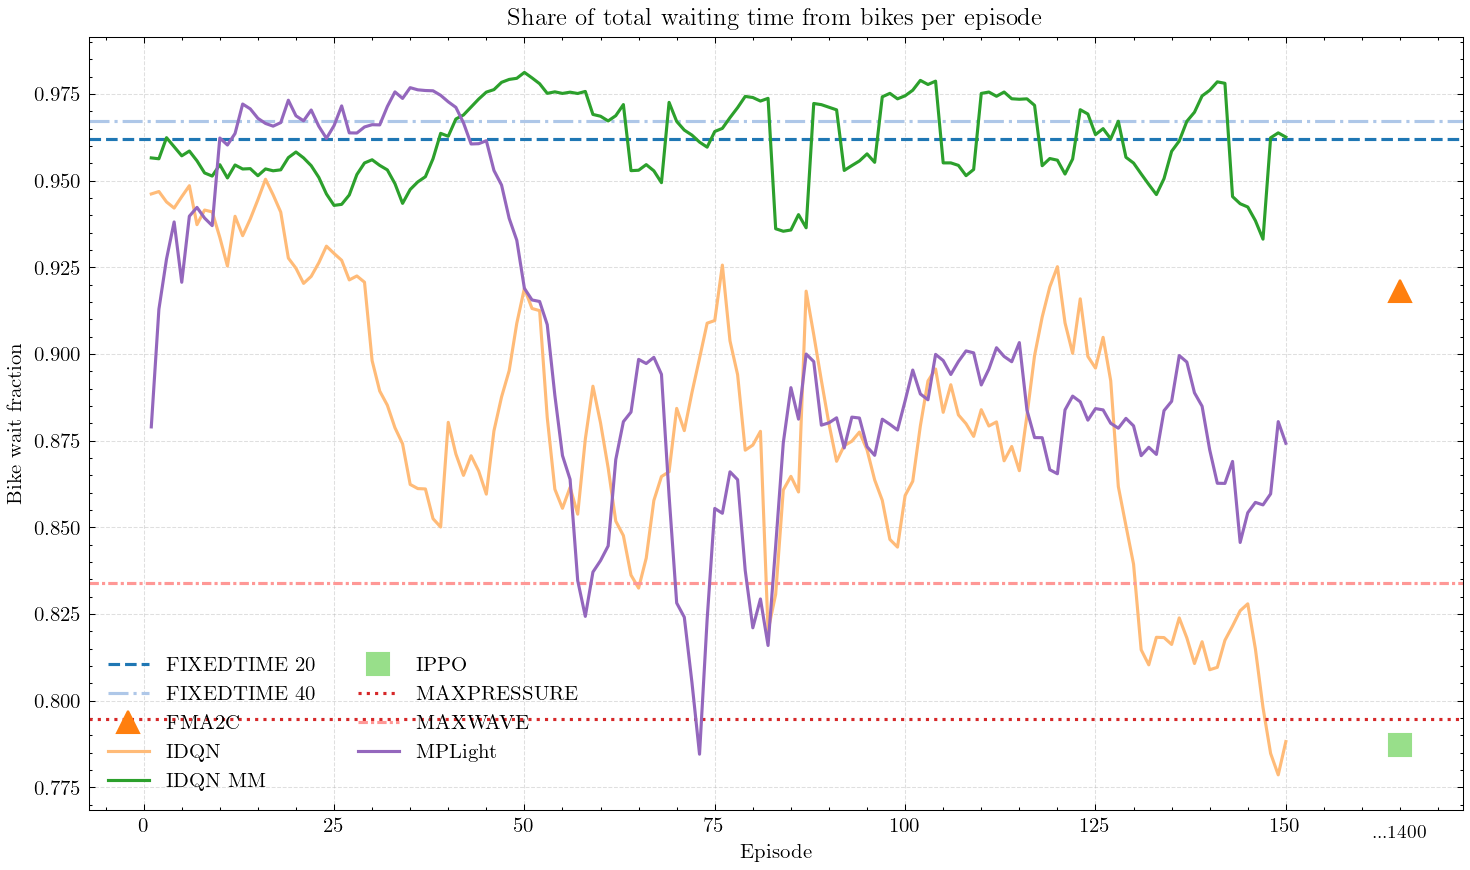
\includegraphics[width=\linewidth]{Figures/chapter04/plotsc2/episode_wait_frac_bike.png}
  \caption{Corridor: fraction of waiting time due to bicycles, per epoch.} \label{fig:frac_wait_bikes_c2}
\end{figure}%
\begin{figure}
  \centering
  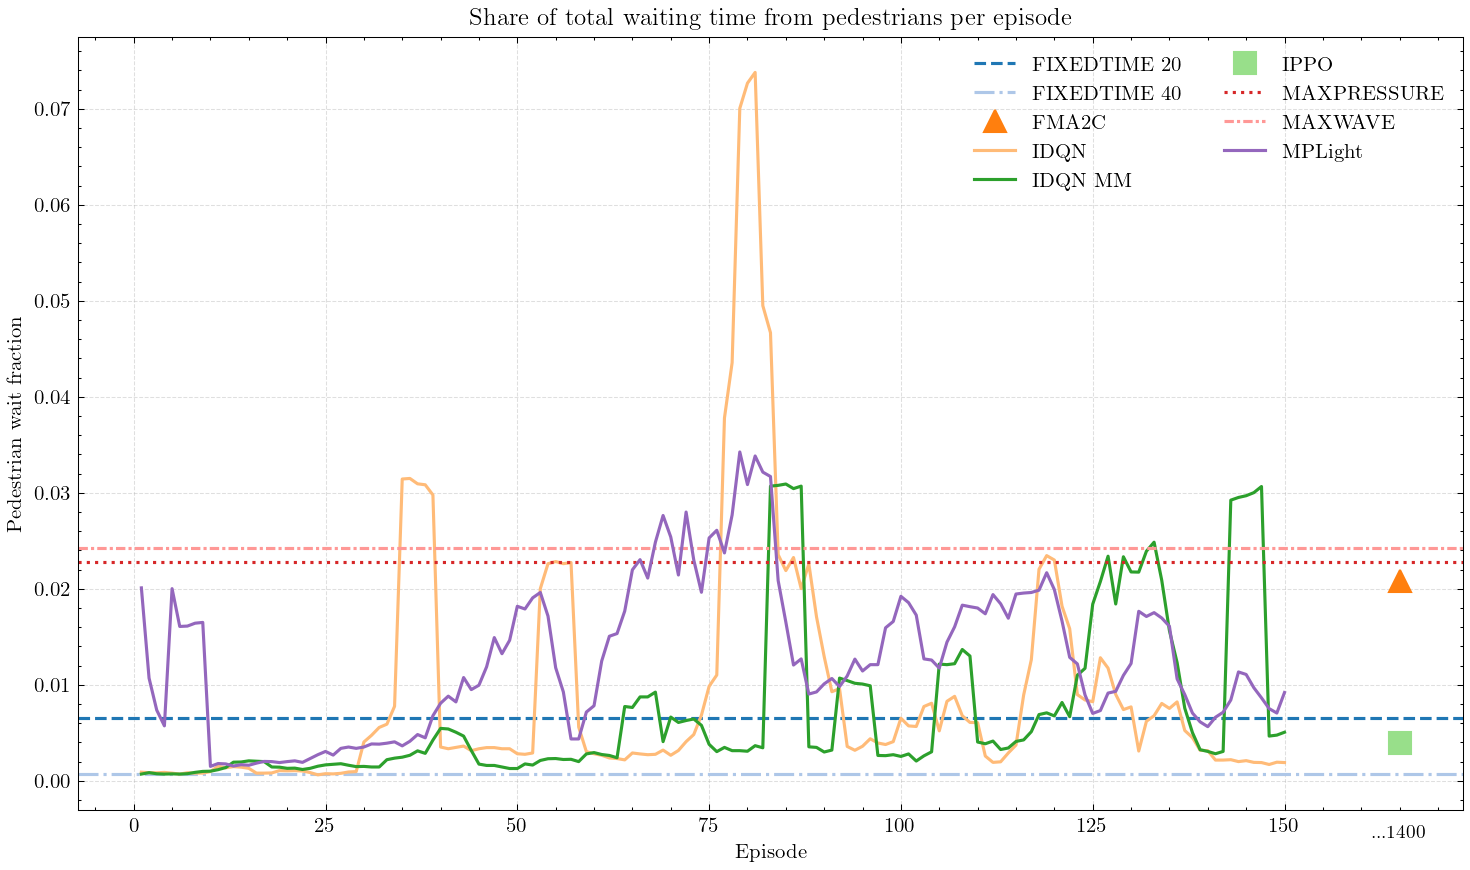
\includegraphics[width=\linewidth]{Figures/chapter04/plotsc2/episode_wait_frac_ped.png}
  \caption{Corridor: fraction of waiting time due to pedestrians, per epoch.} \label{fig:frac_wait_pedestrians_c2}
\end{figure}